% The learning loop of one ring. Adapted from the CAEPIA 2026 slides.
\documentclass[border=0pt]{standalone}
% Shared preamble of the GSO-RL documentation figures.
% Compiled with latex (DVI) + dvisvgm; see ../build.sh.
\def\pgfsysdriver{pgfsys-dvisvgm.def}
\usepackage[T1]{fontenc}
\usepackage{lmodern}
\renewcommand{\familydefault}{\sfdefault}
\usepackage{amsmath, amssymb}
\usepackage{tikz}
\usetikzlibrary{positioning, shapes, arrows.meta, calc, fit, backgrounds}

% Palette
\definecolor{Purple}{RGB}{102, 0, 153}
\colorlet{ColMa}{green!50!black}   % macro-move M1
\colorlet{ColMb}{blue!70!black}    % macro-move M2
\colorlet{ColMc}{orange!85!black}  % macro-move M3
\definecolor{cGa}{RGB}{38, 166, 154}
\definecolor{cGb}{RGB}{229, 96, 76}
\definecolor{cGc}{RGB}{235, 165, 40}
\definecolor{cGd}{RGB}{125, 125, 215}
\definecolor{cGe}{RGB}{190, 60, 150}

% White background so figures stay readable in dark mode. The white rectangle lives on the
% "background" layer; figures draw their own backdrops on "behind", which sits above it.
\pgfdeclarelayer{behind}
\pgfsetlayers{background,behind,main}
\tikzset{every picture/.append style={show background rectangle,
  background rectangle/.style={fill=white, draw=none}, inner frame sep=8pt}}
% NOTE: with dvisvgm, text placed after a \color{...} group inside the same node is misplaced.
% Put differently coloured pieces of text in separate nodes.

\newcommand{\yes}{{\color{green!50!black}\checkmark}}
\newcommand{\nope}{{\color{red!70!black}$\boldsymbol{\times}$}}

% A region: guide with three concentric rings.  \guia[style]{x}{y}{color}{label}
\newcommand{\guia}[5][]{%
  \fill[#4!10, #1] (#2,#3) circle (1.05);
  \fill[#4!20, #1] (#2,#3) circle (0.7);
  \fill[#4!35, #1] (#2,#3) circle (0.35);
  \foreach \r in {0.35,0.7,1.05} \draw[#4, #1] (#2,#3) circle (\r);
  \fill[#4!80!black, #1] (#2,#3) circle (2pt);
  \node[#4!75!black, font=\scriptsize\bfseries, #1] at (#2,#3+1.22) {#5};
}

\begin{document}
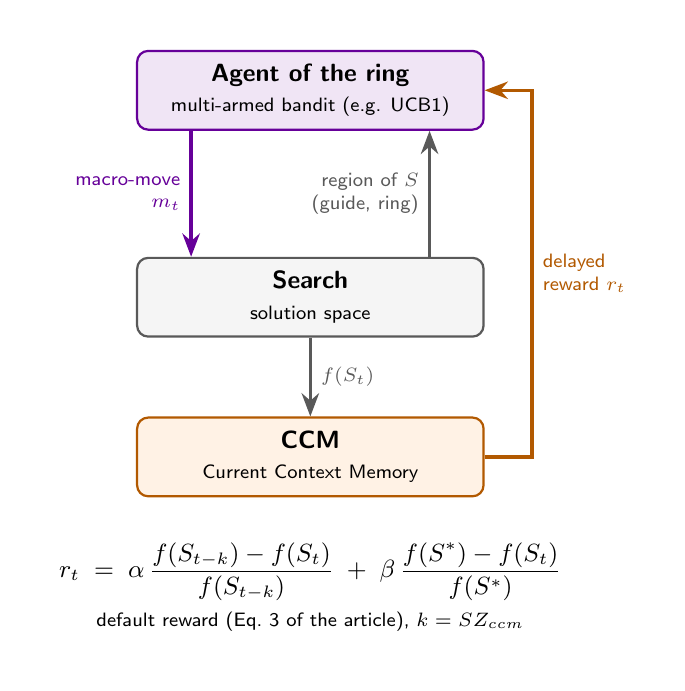
\begin{tikzpicture}[>=Stealth, font=\small,
  box/.style={rectangle, rounded corners, thick, align=center, minimum width=4.4cm, minimum height=1.0cm}]
  \node[box, draw=Purple, fill=Purple!10] (ag) {\textbf{Agent of the ring}\\ \scriptsize multi-armed bandit (e.g. UCB1)};
  \node[box, draw=gray!70!black, fill=gray!8, below=1.6cm of ag] (env) {\textbf{Search}\\ \scriptsize solution space};
  \node[box, draw=orange!70!black, fill=orange!10, below=1.0cm of env] (ccm) {\textbf{CCM}\\ \scriptsize Current Context Memory};

  \draw[->, very thick, Purple] ($(ag.south west)+(0.7,0)$)
    -- node[left, font=\scriptsize, align=right] {macro-move\\ $m_t$} ($(env.north west)+(0.7,0)$);
  \draw[->, very thick, gray!70!black] ($(env.north east)+(-0.7,0)$)
    -- node[left, font=\scriptsize, align=right] {region of $S$\\ (guide, ring)} ($(ag.south east)+(-0.7,0)$);
  \draw[->, very thick, gray!70!black] (env) -- node[right, font=\scriptsize] {$f(S_t)$} (ccm);
  \draw[->, very thick, orange!70!black] (ccm.east) -- ++(0.6,0)
    |- node[pos=0.25, right, font=\scriptsize, align=left] {delayed\\ reward $r_t$} (ag.east);

  \node[below=0.45cm of ccm, font=\small, align=center] (eq)
    {$\displaystyle r_t \;=\; \alpha\,\frac{f(S_{t-k}) - f(S_t)}{f(S_{t-k})} \;+\; \beta\,\frac{f(S^*) - f(S_t)}{f(S^*)}$\\[3pt]
     \scriptsize default reward (Eq.~3 of the article), $k = SZ_{ccm}$};
\end{tikzpicture}
\end{document}
